\documentclass[../../main.tex]{subfiles}

\graphicspath{{../../image/}{../../figure/}}

\begin{document}

\section{多模态 Transformer}\label{section:ch12-多模态Transformer}

虽然 Transformer 最初是作为处理顺序语言数据的递归网络的替代品而开发的，但 Transformer 模型已在深度学习的几乎所有领域得到普及。事实证明，它们是通用模型，因为它们对输入数据的假设很少，而对卷积网络的等变性和局部性有很强的假设。由于其通用性，Transformer 已成为处理许多不同模态数据（包括文本、图像、视频、点云和音频数据）的最先进技术，并已用于这些领域中每个领域的判别和生成应用（参见\cref{chapter:ch10-卷积网络}）。Transformer 层的核心架构在不同时期和不同应用中保持相对稳定。因此，能够在自然语言以外的领域使用 Transformer 的关键创新主要集中在输入和输出的表示及编码方面。

能够处理多种不同数据的单一架构有一个巨大优势，就是能使多模态计算变得相对简单。在这种情况下，多模态指的是将两种或两种以上类型的数据结合在一起。例如，我们可能希望根据文字提示生成图像，或者设计一个能将摄像头、雷达和麦克风等多个传感器捕获的信息结合起来的机器人。重要的是，如果我们能对输入进行 token 化并对输出 token 进行解码，那么我们就有可能使用 Transformer。

\subsection{视觉 Transformer}\label{subsection:ch12-视觉Transformer}

Transformer 已成功应用于计算机视觉领域，并在许多任务中有着不俗的表现。判别任务最常见的选择是标准 Transformer，其在视觉领域又称视觉 Transformer（Vision Transformer，简称 ViT）（Dosovitskiy et al., 2020）。在使用 Transformer 时，我们需要决定如何将输入图像转换为 token，最简单的选择是将每个像素作为一个 token 并按照线性投影进行转换。然而，标准 Transformer 实现所需的内存与输入 token 的数量成二次方增长关系，因此这种方法通常是不可行的。相反，最常见的分词方法是将图像分割成一组大小相同的小块。假设图像的尺寸为 $\mathbf{x}\in\mathbb{R}^{H\times W\times C}$，其中 $H$ 和 $W$ 分别指的是图像的高度和宽度（以像素为单位），$C$ 是通道数（R、G、B 三种颜色的通道数通常为 $3$）。每幅图像被分割成大小为 $P\times P$ 的非重叠小块（$P=16$ 是常见的选择），然后“平铺”成一维向量，这样就得到了图像尺寸的另一种表示 $\mathbf{x}_p\in\mathbb{R}^{N\times(P^{2}C)}$，其中 $N=HW/P^{2}$ 是一幅图像的小块总数。用于分类任务的视觉 Transformer 的架构如\cref{figure:ch12-ViT}所示。

\begin{figure}[htbp]
  \centering
  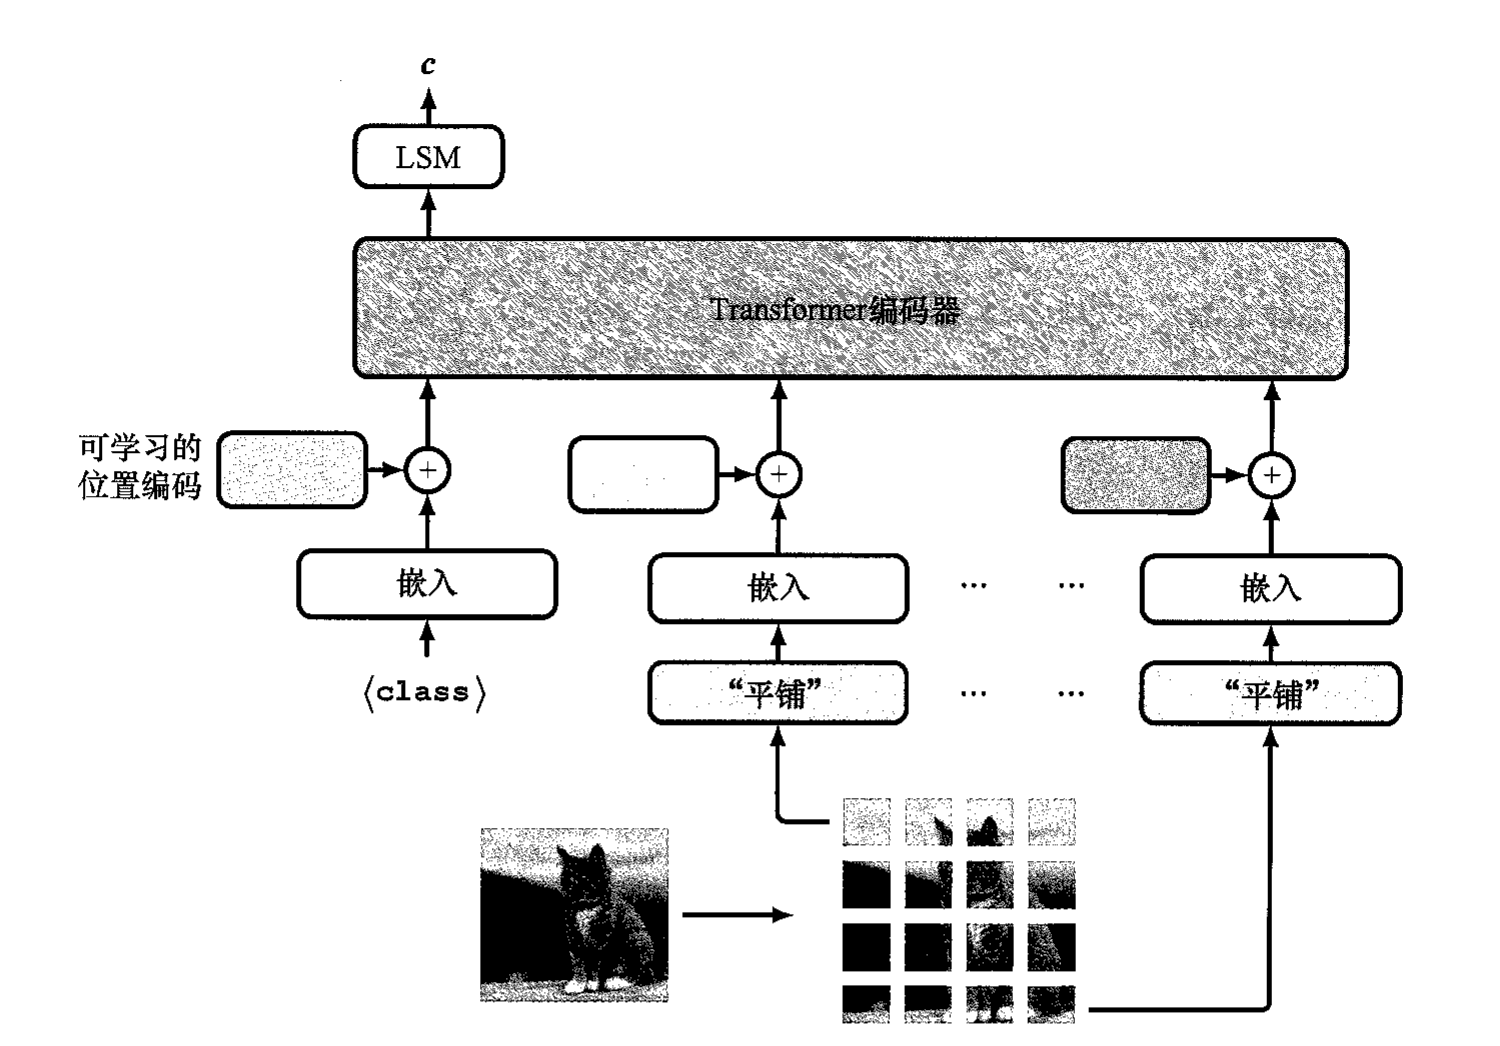
\includegraphics[width=0.85\textwidth]{ch12-fig367-vit.png}
  \caption{用于分类任务的视觉 Transformer 的架构。此处将一个可学习的 token $\langle\mathrm{class}\rangle$ 作为额外的输入，相关的输出由一个具有 softmax 激活函数的线性层（记作 LSM）进行转换，从而得到最终的类-向量输出 $\mathbf{c}$。}
  \label{figure:ch12-ViT}
\end{figure}

另一种分词方法是将图像输入一个小型卷积神经网络（参见\cref{chapter:ch10-卷积网络}）。这样就可以对图像进行采样，从而得到数量可控的 token，每个 token 由一个网络输出表示。例如，一个典型的 ResNet18 编码器将在高度和宽度两个维度对图像进行 8 倍的下采样，所得到的 token 数量是像素数量的 $1/64$。

我们还需要一种在 token 中编码位置信息的方法。我们可以构建明确的位置嵌入，对图像小块的二维位置信息进行编码。但在实践中，这一般不会提高性能，因此最常见的做法是只使用习得的位置嵌入。与用于自然语言的 Transformer 不同，视觉 Transformer 通常将固定数量的 token 作为输入，从而避免了习得的位置编码无法泛化到不同大小的输入的问题。

视觉 Transformer 的架构设计与卷积神经网络截然不同。虽然卷积神经网络中会产生强归纳偏置，但视觉 Transformer 中唯一的二维归纳偏置是用于 token 化输入的小块造成的。因此，视觉 Transformer 通常比卷积神经网络需要更多的训练数据，因为它必须从头开始学习图像的几何特性。不过，由于对输入的结构没有很强的假设，视觉 Transformer 通常能够收敛到更高的精度。这再次说明了归纳偏置与训练数据规模之间需要权衡（Sutton, 2019）。

\begin{definition}[图像块 token 化]\label{definition:ch12-图像块分词}
设图像 $\mathbf{x}\in\mathbb{R}^{H\times W\times C}$，小块边长为 $P$（$P$ 整除 $H,W$）。把图像划分为 $N=HW/P^{2}$ 个互不重叠的 $P\times P\times C$ 小块，并将每块展平为长度 $P^{2}C$ 的向量，得到矩阵 $\mathbf{x}_p\in\mathbb{R}^{N\times(P^{2}C)}$，再经可学习的线性投影映射到 $D$ 维，则称这一过程为图像的\textbf{块 token 化}。
\end{definition}

% SUPPLEMENT: parent=definition:ch12-图像块分词; kind=motivation; location=紧随其后的 remark（重构新增）
\begin{remark}（重构新增）
块 token 化的动机是复杂度：若以像素为 token，$N=HW$ 可达 $10^{5}$ 量级，注意力的 $O(N^{2}D)$ 代价无法承受（见\cref{proposition:ch12-计算复杂度}）；以 $16\times16$ 小块为单位，$224\times224$ 的图像得到 $N=196$ 个 token，复杂度降到可行范围。条件“$P$ 整除 $H,W$”保证划分无剩余，否则需要补齐。这一设计也解释了 ViT 的归纳偏置为何弱于卷积网络：卷积核天然编码了“局部性”与“平移等变”，而块 token 化只保留了“局部小块”这一条，其余几何关系必须由数据和位置编码学出来，因此需要更大规模的预训练数据。线性投影的维度 $D$ 与语言模型一致，使同一套 Transformer 层可以直接复用。
\end{remark}

除了图像块的 token，我们还为输入序列增加了一个可学习的分类 token（用 $\mathbf{c}$ 表示），如\cref{figure:ch12-ViT}所示。我们将整个序列输入一个仅编码器 Transformer（参见\cref{subsection:ch12-编码器型Transformer}）。这个序列有 196 个图像 token 和 1 个分类 token，其中分类 token 最终编码了图像的整体表示，可用于下游分类。在经过 $L$ 个 Transformer 层处理后，我们可以从最终输出序列中提取出分类 token，并使用全连接层进行处理以执行分类任务。\cref{figure:ch12-ViT}所示的视觉 Transformer 架构使用了 $L=12$ 层、维度为 $D=768$ 和 12 个注意力头，总共有大约 8600 万个可学习参数。

值得注意的是，虽然视觉 Transformer 是在 ImageNet 数据集上进行预训练的，但它们在小型数据集上的表现通常不如卷积网络（例如 ResNet），因为它们没有内建的图像结构归纳偏置。当在大型数据集上进行预训练时，视觉 Transformer 的性能优于卷积网络。因此，卷积网络通常可以作为特征提取器，为 Transformer 提供输入。

\subsection{图像生成 Transformer}\label{subsection:ch12-图像生成Transformer}

在语言领域，Transformer 在用作合成文本的自回归生成式模型时取得了令人瞩目的成果。因此，人们自然会问是否也可以使用 Transformer 来合成逼真的图像。由于自然语言本身具有顺序性，因此其非常适合自回归框架，而图像的像素没有自然顺序，因此自回归解码是否有用并不那么直观。然而，只要首先定义变量的某种排序，任何分布都可以分解为条件式的乘积（参见\cref{section:ch11-序列模型}）。有序变量 $x_1,\cdots,x_N$ 的联合分布可以写成
\begin{align}
p(x_1,\cdots,x_N)=\prod_{n=1}^{N}p(x_n\mid x_1,\cdots,x_{n-1})
\label{align:ch12-图像自回归}
\end{align}

这种分解是完全通用的，对各个条件分布 $p(x_n\mid x_1,\cdots,x_{n-1})$ 的形式没有任何限制。

对于一幅图像，我们可以选择 $x_n$ 作为 R、G、B 值的三维向量来表示第 $n$ 个像素。现在我们需要确定像素的排序，其中一种使用广泛的排序方式叫栅格扫描（raster scan），如\cref{figure:ch12-栅格扫描}所示。使用基于栅格扫描排序的自回归模型生成图像如\cref{figure:ch12-图像自回归采样}所示。

\begin{figure}[htbp]
  \centering
  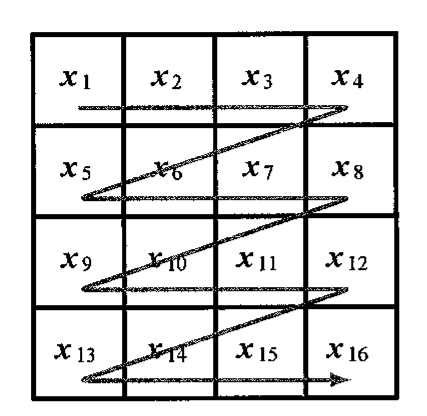
\includegraphics[width=0.3\textwidth]{ch12-fig12-23-raster-scan.png}
  \caption{定义二维图像中像素的特定线性排序的栅格扫描示意图。}
  \label{figure:ch12-栅格扫描}
\end{figure}

\begin{figure}[htbp]
  \centering
  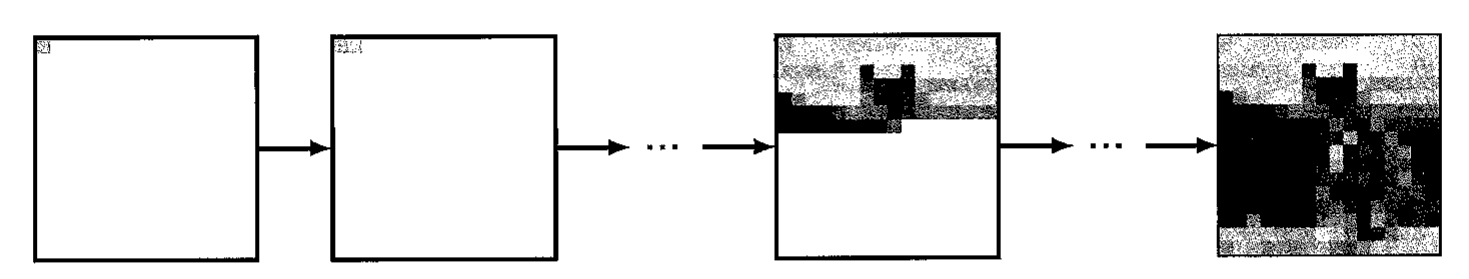
\includegraphics[width=0.85\textwidth]{ch12-fig12-24-autoregressive-image.png}
  \caption{从自回归模型中进行图像采样的示意图。按栅格扫描顺序，第一个像素从边缘分布 $p(x_1)$ 中采样，第二个像素从条件分布 $p(x_2\mid x_1)$ 中采样，以此类推，直至得到一幅完整的图像。}
  \label{figure:ch12-图像自回归采样}
\end{figure}

请注意，图像自回归生成式模型的使用早于 Transformer 的引入。例如，PixelCNN（Oord et al., 2016）和 PixelRNN（Oord, Kalchbrenner, and Kavukcuoglu, 2016）使用了定制的遮掩卷积层，其保留了\eqref{align:ch12-图像自回归}右侧相应项为每个像素定义的条件独立性。

使用连续值的图像表示可以很好地完成判别任务。不过，使用离散表示法生成图像的效果要好得多。通过最大似然法习得的连续条件分布，例如负对数似然函数为平方和误差函数的Gauss分布，往往会学习到训练数据的均值，从而导致图像模糊（参见\cref{section:ch04-决策理论}）。相反，离散分布可以轻松处理多模态问题。例如，\eqref{align:ch12-图像自回归}中的条件分布 $p(x_n\mid x_1,\cdots,x_{n-1})$ 可能会得出一个像素应该是黑色或白色的结论，而回归模型可能会得出该像素应该是灰色的结论。

然而，使用离散空间也会带来挑战。图像像素的 R、G、B 值通常至少用 8 位精度来表示，因此每个像素都有 $2^{24}\approx1600$ 万个可能值。在维度如此高的空间中学习条件 softmax 分布是不可行的。

解决高维度问题的一种方法是使用向量量化（vector quantization）技术，它可以视为一种数据压缩形式。假设我们有一组数据向量 $\mathbf{x}_1,\cdots,\mathbf{x}_N$，其中每个向量的维度为 $D$，它可能代表图像像素。然后我们引入一组 $K$ 个码本向量 $\mathcal{C}=\mathbf{c}_1,\cdots,\mathbf{c}_K$，它们的维度也是 $D$，且通常情况下 $K\ll D$。接下来，我们根据某种相似度量（通常是欧几里得距离），将每个数据向量近似为其最近的码本向量（codebook vector），从而
\begin{align}
\mathbf{x}_n\to\underset{\mathbf{c}_k\in\mathcal{C}}{\arg\min}\left\|\mathbf{x}_n-\mathbf{c}_k\right\|^{2}
\label{align:ch12-向量量化}
\end{align}

由于有 $K$ 个码本向量，我们可以用一个独热编码的 $K$ 维向量来表示每个 $\mathbf{x}_n$，而且由于我们可以选择 $K$ 的值，因此我们可以通过使用较大的 $K$ 值来更准确地表示数据，或使用较小的 $K$ 值来更大程度地压缩数据，从而进行两者之间的权衡。

\begin{definition}[向量量化]\label{definition:ch12-向量量化}
设码本 $\mathcal{C}=\{\mathbf{c}_1,\cdots,\mathbf{c}_K\}\subset\mathbb{R}^{D}$。映射 $Q:\mathbb{R}^{D}\to\mathcal{C}$，$Q(\mathbf{x})=\arg\min_{\mathbf{c}\in\mathcal{C}}\|\mathbf{x}-\mathbf{c}\|$，称为\textbf{向量量化}（vector quantization）；每个数据点用它最近码本的索引表示，索引再经独热编码送入后续模型。
\end{definition}

% SUPPLEMENT: parent=definition:ch12-向量量化; kind=motivation; location=紧随其后的 remark（重构新增）
\begin{remark}（重构新增）
向量量化的作用是把“连续高维取值”变成“有限字典上的离散符号”，从而让 softmax 型语言模型可以直接用于像素。$K$ 的选择就是保真度与可学习性的权衡：$K$ 太小，量化误差大，重建图像失真；$K$ 太大，每个码本被数据覆盖的机会变小，softmax 参数难以估计（与\cref{proposition:ch12-词袋最大似然}中零频问题同源）。$\arg\min$ 不可微是这里的结构性障碍——梯度无法穿过“取最近邻”这一步，因此实践中需要用直通估计（straight-through estimator）把梯度近似地复制到编码器一侧。\eqref{align:ch12-向量量化}定义的是硬分配；若改用 softmax 给出各码本的概率，就得到软量化，这与注意力的软硬之分是同一思想。
\end{remark}

我们可以将原始图像的像素映射到低维码本空间，然后训练自回归 Transformer 以生成一组码本向量，并通过用相应的 $D$ 维码本向量 $\mathbf{c}_k$ 替换每个码本索引 $k$，将这组码本向量映射回原始图像空间。

自回归 Transformer 最早应用于 ImageGPT（Chen, Radford, et al., 2020）中的图像。此处，每个像素都可以视为一组离散的三维颜色码本向量之一，每个三维颜色码本向量都与颜色空间的 $k$ 均值聚类中的一个聚类相对应（参见\cref{chapter:ch15-离散潜变量}）。因此，独热编码可以提供离散 token（类似于语言 token），并允许 Transformer 以与语言模型相同的方式进行训练，以实现下一个 token 分类目标。这是表示学习的一个强大目标（参见\cref{subsection:ch06-表示学习}），可用于后续微调（同样以类似于语言建模的方式进行）。

然而，直接使用单个像素作为 token 可能会导致计算成本过高，因为每个像素都需要进行一次前向传递，这意味着训练和推理的效率都会随着图像分辨率的提高而降低。此外，使用单个像素作为输入意味着必须使用低分辨率图像，以便在栅格扫描后期解码像素时提供合理的上下文长度。正如我们在视觉 Transformer 中看到的那样，最好使用图像的小块而不是像素作为 token，因为这样 token 的数量会大大减少，从而有利于处理更高分辨率的图像。和以前一样，由于条件分布可能具有多模态性，我们需要使用 token 值的离散空间。于是再次出现维度挑战，由于维度与小块中像素的数量成指数关系，因此小块的维度比单个像素的维度大得多。例如，即使只有代表黑色和白色两种可能像素的 token，以及大小为 $16\times16$ 的小块，我们也会有一个内含 $2^{256}\approx10^{77}$ 个小块的 token 字典。

我们再次使用向量量化技术来解决维度挑战。简单的聚类（如 $k$ 均值聚类）方法或更复杂的方法（如全卷积网络）（Oord, Vinyals, and Kavukcuoglu, 2017; Esser, Rombach, and Ommer, 2020），甚至包括视觉 Transformer（Yu et al., 2021），都可以用来从图像小块数据集中习得码本向量。将每个小块映射到离散的代码集，之后再映射回来的一个问题是，向量量化是一种不可微分操作。幸运的是，我们可以使用一种称为直通梯度估计的技术（Bengio, Léonard, and Courville, 2013），这是一种简单的近似法，只需要在反向传播过程中通过不可微分函数复制梯度即可。

使用自回归 Transformer 生成图像也可以扩展到生成视频，方法是将视频视为这类向量量化 token 的一个长序列（Rakhimov et al., 2020; Yan et al., 2021; Hu et al., 2023）。

\subsection{音频数据}\label{subsection:ch12-音频数据}

接下来让我们看看 Transformer 在音频数据中的应用。声音通常以波形的形式存储，它们可以通过在固定时间间隔内测量气压的振幅来获得。虽然这种波形可以直接作为深度学习模型的输入，但在实践中，将其预处理为梅尔频谱（mel spectrogram）更为有效。这是一个矩阵，其中的列代表时间步，行代表频率。这些频段遵循标准惯例（标准惯例是通过主观评估选择的），从而使得连续频率之间的感知差异相等（“mel”一词来源于旋律）。梅尔频谱如\cref{figure:ch12-梅尔频谱}所示。

\begin{figure}[htbp]
  \centering
  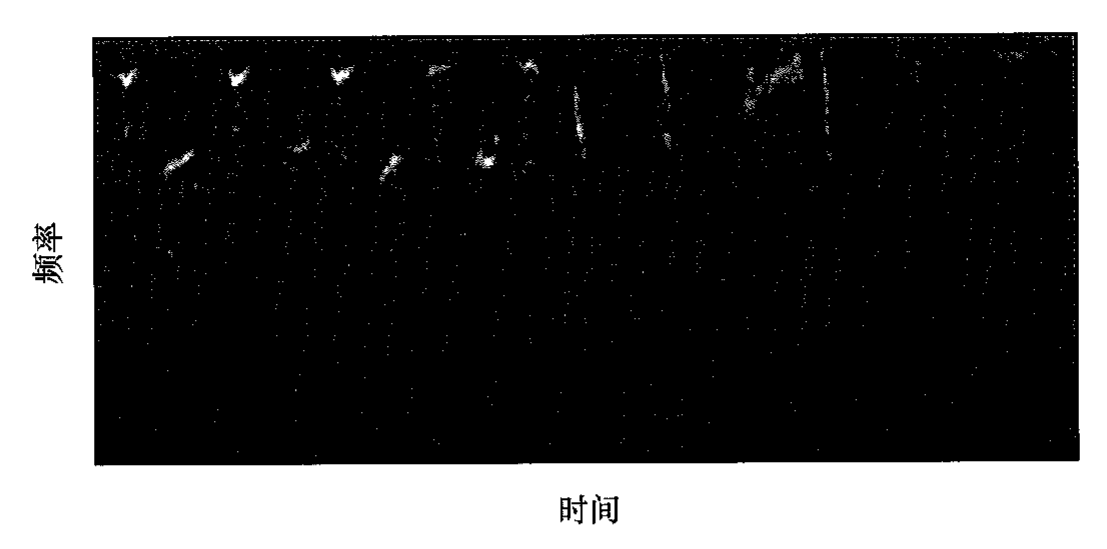
\includegraphics[width=0.6\textwidth]{ch12-fig12-25-mel-spectrogram.png}
  \caption{座头鲸叫声的梅尔频谱（librosa 开发团队版权所有 \copyright 2013–2023）。}
  \label{figure:ch12-梅尔频谱}
\end{figure}

Transformer 在音频领域的一个应用是分类，旨在将音频片段归入若干预定义类别之一。例如，AudioSet 数据集（Gemmeke et al., 2017）就是一个使用广泛的基准，其中包含“汽车”“动物”“笑声”等类。在 Transformer 出现之前，最先进的音频分类方法是将梅尔频谱作为图像进行处理，并将其作为卷积神经网络的输入（参见\cref{chapter:ch10-卷积网络}）。不过，虽然卷积神经网络擅长理解局部关系，但它的一个缺点是难以处理远距离依赖关系，而这在处理音频时可能非常重要。

正如 Transformer 取代递归神经网络成为自然语言处理领域的最先进技术一样，Transformer 在音频分类等任务中也开始取代卷积神经网络。例如，如\cref{figure:ch12-编码器BERT}所示，编码器型 Transformer 与用于语言和视觉的 Transformer 结构相同，可用于预测音频输入的类（Gong, Chung, and Glass, 2021）。此处，梅尔频谱可以视为图像，然后进行 token 化。具体做法是以类似于视觉 Transformer 的方式将图像分割成不同的小块，可能会有一些重叠，以避免丢失任何重要的邻域关系。然后对每个小块进行扁平化处理，也就是将它们转换为一维数组，在本例中长度为 $256$。之后为每个 token 添加唯一的位置编码，并附加特定的 token $\langle\mathrm{class}\rangle$，接下来通过编码器型 Transformer 输入 token。我们可以使用一个线性层和一个 softmax 激活函数对最后一个转换层中与输入 token $\langle\mathrm{class}\rangle$ 相对应的输出 token 进行解码，并使用交叉熵损失对整个模型进行端到端训练。

\subsection{文本语音转换}\label{subsection:ch12-文本语音转换}

分类并不是深度学习（更具体地说是 Transformer 架构）在音频领域带来革命性变化的唯一任务。Transformer 成功地合成了模仿特定说话者声音的语音这一事实再次证明了 Transformer 的多功能性，而 Transformer 在这项任务中的应用则是关于如何在新环境中应用 Transformer 的一项内容十分丰富的案例研究。

生成与给定文本段落相对应的语音叫作文本语音合成（text-to-speech synthesis）。一种更传统的方法是收集特定说话者的录音，然后训练一个监督回归模型，从而根据相应的转录文本预测语音输出（可能采用梅尔频谱的形式）。在推理过程中，我们希望将合成语音的文本作为输入，由此产生的梅尔频谱输出则可以解码回音频波形，因为这是一个固定的映射。

不过，这种方法有 3 个主要不足。首先，如果我们在低层次上预测语音，例如使用叫作音素（phoneme）的子词组件，则需要更大的上下文来使生成的句子听起来流畅。但是，如果我们预测更长的片段，那么可能的输入空间就会显著增大；要达到良好的泛化效果，我们可能需要大量的训练数据。其次，这种方法不能在不同说话者之间传递知识，因此每个新的说话者都需要大量数据。最后，这实际上是一个生成建模任务，因为给定的说话者和文本对有多个正确的语音输出，所以回归可能并不合适，回归倾向于对目标值进行平均（参见\cref{section:ch04-决策理论}）。

相反，如果我们将语音数据与自然语言同等对待，并将文本语音合成作为一项条件语言建模任务，那么我们就能以与基于文本的大语言模型大致相同的方式训练该模型。此时我们需要解决两个主要的实现细节问题。首先是如何对训练数据进行 token 化并对预测值进行解码，其次是如何根据说话者的声音对模型进行调节。

Vall-E（Wang et al., 2023）是一种利用 Transformer 和语言建模技术进行文本语音合成的方法。只需要几秒样本语音，就能将新文本映射成新说话者的语音。语音数据通过向量量化获得的字典或码本（codebook）被转换成一组离散 token（参见\cref{subsection:ch12-图像生成Transformer}），我们可以将这类 token 视为类似于自然语言领域的独热编码 token。输入由文本段落中的文本 token 组成，而用于训练的目标输出则由相应的语音 token 组成。如\cref{figure:ch12-VallE}所示，来自同一说话者的一小段无关语音的附加语言 token 会被添加到输入文本 token 中。通过加入来自许多不同说话者的额外语音 token，系统可以在模仿这些额外语音 token 所代表的声音时学习朗读一个文本段落。训练完成后，系统就可以显示新的文本，以及从新的说话者那里捕捉到的一段简短语音中的音频 token，并使用训练时的相同码本对输出 token 进行解码，以创建语音波形。这样系统就能用新说话者的声音合成与输入文本相对应的语音。

\begin{figure}[htbp]
  \centering
  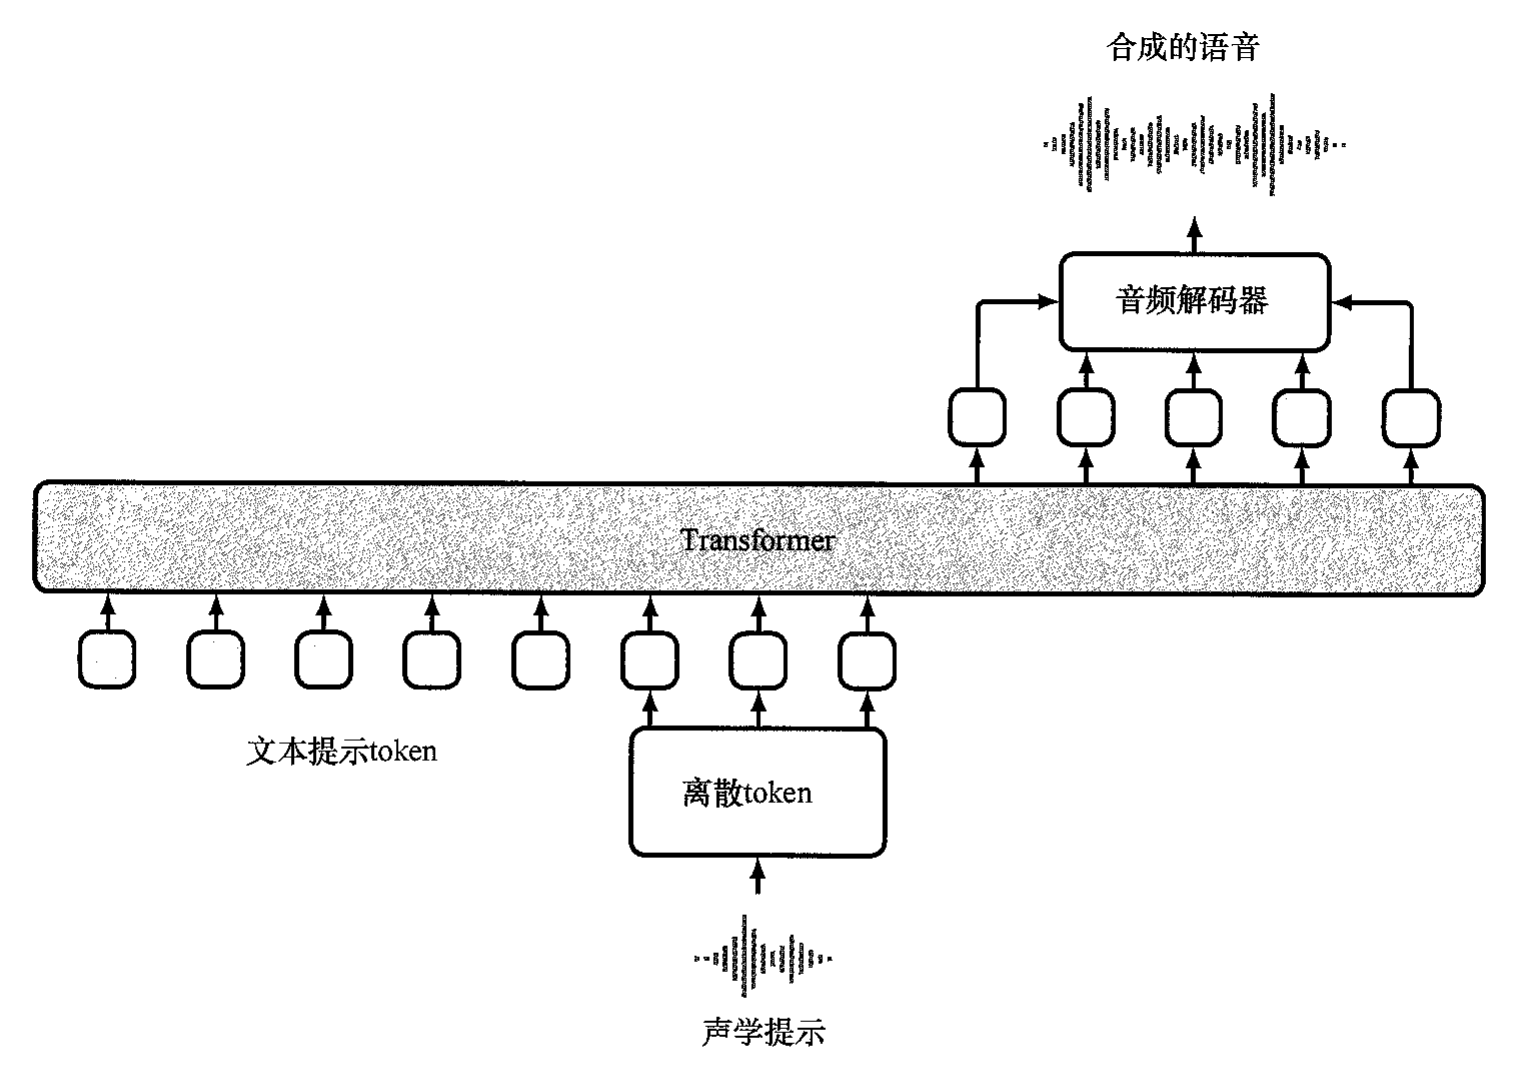
\includegraphics[width=0.85\textwidth]{ch12-fig12-26-valle.png}
  \caption{Vall-E 高级架构图。Transformer 模型的输入包括文本提示 token（提示模型合成的语音应包含哪些词）和声学提示 token（确定说话者的风格和语调信息）。使用习得的解码器将采样的模型输出 token 解码为语音。为简单起见，这里没有显示位置编码和线性投影。}
  \label{figure:ch12-VallE}
\end{figure}

\subsection{视觉和语言 Transformer}\label{subsection:ch12-视觉和语言Transformer}

我们已经了解了如何生成文本、音频和图像的离散 token，接下来的问题是，我们是否可以用一种模态的输入 token 和另一种模态的输出 token 来训练模型。或者说，我们是否可以将不同模态的输入或输出抑或它们两者结合起来，在这里，我们将重点讨论文本和视觉数据的组合，因为这是研究最广泛的示例，但原则上，此处讨论的方法也可应用于其他输入和输出模态的组合。

第一个要求是，我们要有一个庞大的数据集来进行训练。LAION-400M 数据集（Schuhmann et al., 2021）极大地促进了文生图和图生文的研究，该数据集与 ImageNet 数据集一样，对深度图像分类模型的发展起着关键作用。文生图实际上与我们迄今为止研究过的无条件图像生成很相似，只不过我们还允许模型将文本信息作为输入，为生成过程提供条件。使用 Transformer 时，进行文生图非常简单，因为我们只需要在解码每个图像 token 时提供文本 token 作为额外输入即可。

这种方法也可视为将文生图问题看作序列到序列的语言建模问题，如机器翻译，只不过目标 token 是离散的图像 token 而不是语言 token。因此，选择一个完整的编码器-解码器 Transformer 模型是合理的，如\cref{figure:ch12-序列到序列}所示，其中 $\mathbf{X}$ 对应于输入文本 token，$\mathbf{Y}$ 对应于输出图像 token。一个名为 Parti 的模型（Yu et al., 2022）就采用了这种方法，其中 Transformer 可扩展至 200 亿个参数，同时随着模型规模的增大，性能也得到了持续改善。

在使用预训练的语言模型并对其进行修改或微调，以使其也能接收视觉数据作为输入方面，业界也开展了大量研究（Alayrac et al., 2022; Li et al., 2022）。这些研究主要使用定制架构和连续值图像 token，因此并不适合同时生成视觉数据。此外，如果我们希望加入音频 token 等新模态，也不能直接使用它们。尽管这是向多模态迈出的一步，但我们还是希望将文本 token 和图像 token 同时用作输入和输出。最简单的方法是将所有内容都视为一组 token，就像自然语言一样，但使用的字典是语言 token 字典和图像 token 码本的组合。这样我们就可以将任何视听数据流简单地视为一组 token 了。

在 CM3（Aghajanyan et al., 2022）和 CM3Leon（Yu et al., 2023）中，语言建模的一种变体用于对 HTML 文档进行训练，这些文档包含从在线资源中获取的图像和文本数据。当大量的训练数据与可扩展的架构相结合时，模型就会变得非常强大。此外，训练的多模态性质意味着模型非常灵活。这类模型不仅能够完成许多原本需要特定任务模型架构和训练机制才能完成的任务，如文生图、图生文、图像编辑、文本补全等，还能够完成普通语言模型所能完成的任何任务。\cref{figure:ch12-CM3Leon}给出了 CM3Leon 模型在文本和图像联合空间中执行各种不同任务的示例。

\begin{figure}[htbp]
  \centering
  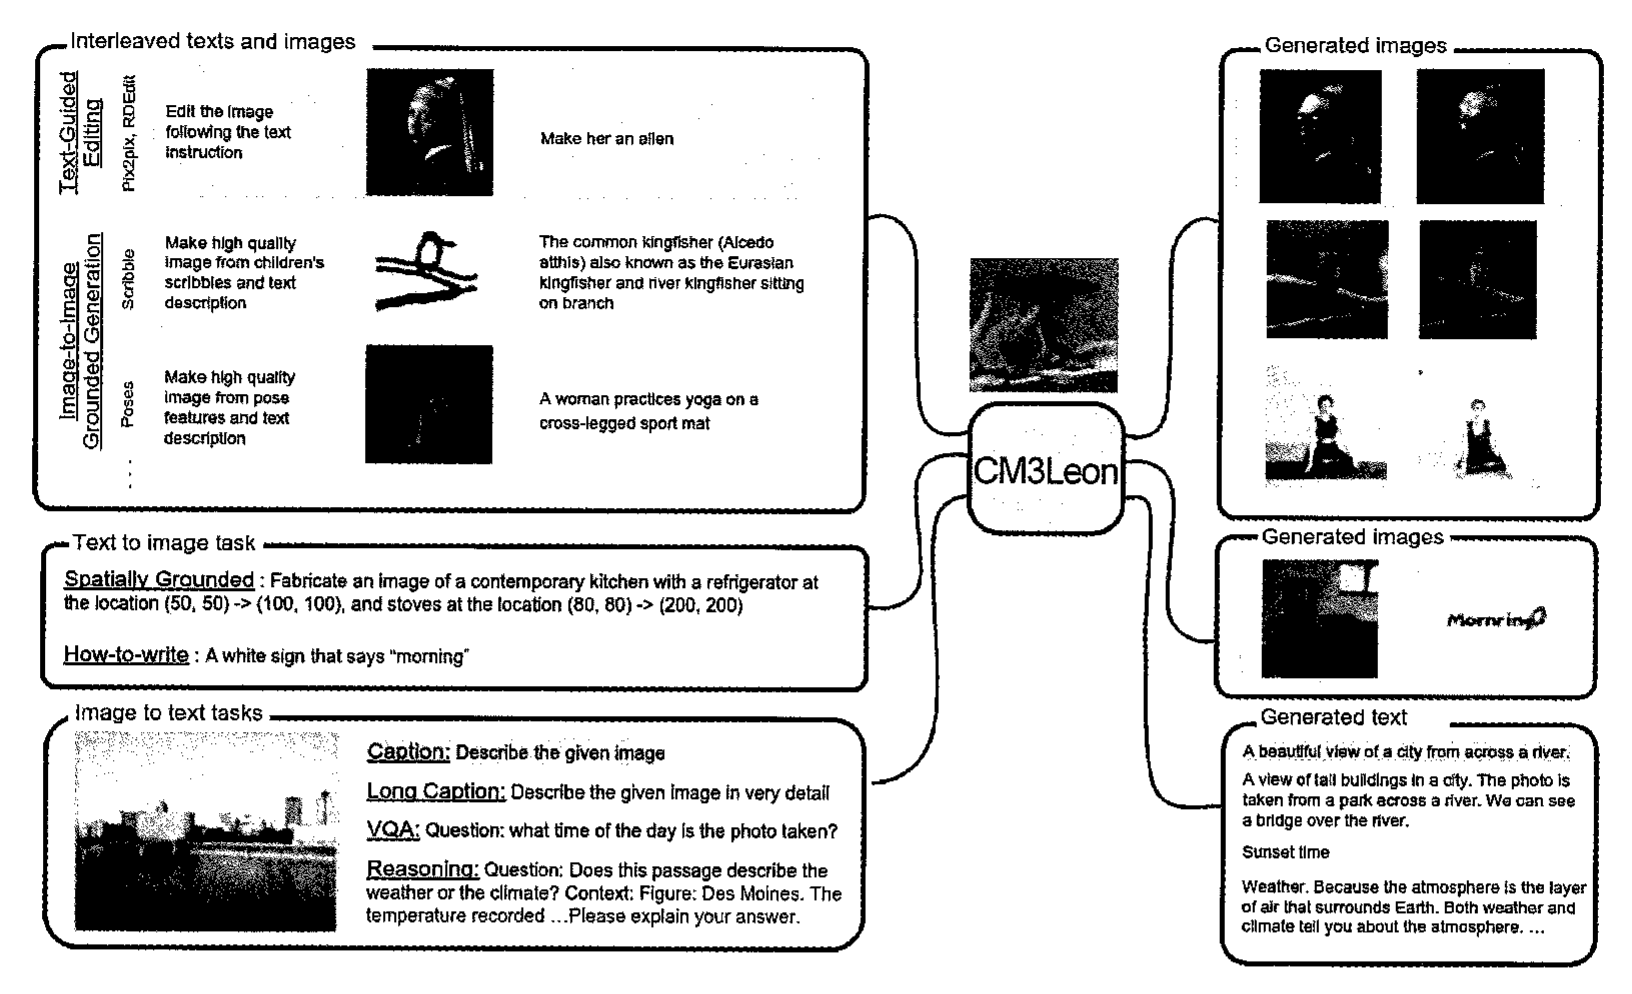
\includegraphics[width=0.95\textwidth]{ch12-fig12-27-cm3leon.png}
  \caption{CM3Leon 模型在文本和图像联合空间中执行各种不同任务的示例[经 Yu 等人（2023）授权使用]。}
  \label{figure:ch12-CM3Leon}
\end{figure}

\end{document}
